\section{Overview}

\subsection{A Story in Pictures}
\begin{frame}
  \centering
  
\includegraphics[height=0.95\textheight]{phd1531}
  \footnote{http://phdcomics.com/comics/archive.php?comicid=1531}
\end{frame}

\begin{frame}
  \centering
  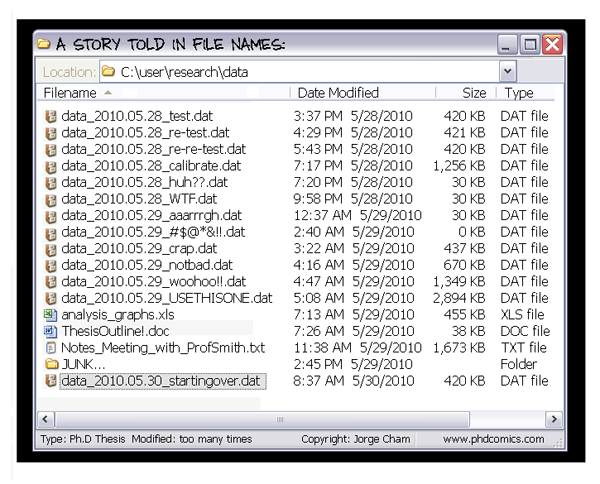
\includegraphics[height=0.95\textheight]{phd1323}
  \footnote{http://phdcomics.com/comics/archive.php?comicid=1323}
\end{frame}

\subsection{Tracking History}

\begin{frame}[fragile]
The history of a project can be viewed as a series of changes:
\small
\begin{verbatim}
* data_2010.05.30-USETHISONE.dat
|
* data_2010.05.30-whoohoo!.dat
|
* data_2010.05.29-##$#$!.dat
|
* data_2010.05.29-aaaaargh.dat
|
* data_2010.05.28-calibrate.dat
|
* data_2010.05.28-re-retest.dat
|
* data_2010.05.28-retest.dat
|
* data_2010.05.28-test.dat
\end{verbatim}
\end{frame}

\begin{frame}
  \frametitle{Tracking Changes}
  \begin{itemize}
    \item A unique identifier
    \item What changed?
    \item When did it change?
    \item Who changed it?
    \item Why did it change?
    \item[]
    \item Difficult to manually track multiple files
  \end{itemize}
\end{frame}

\begin{frame}
  \frametitle{Git: A Version Control System}
  \begin{itemize}
    \item A snapshot of the working directory is taken and \emph{commit}ed to
      the git data base.
    \item Unique identifier: SHA-1 (determined by the files, the author, date,
      description of change, and the prior history)
    \item What changed: git diff
    \item Who changed it: git blame
    \item Why did it change: git log
    \item[]
    \item for example:
  \end{itemize}
\end{frame}
